\chapter{Related Research}
 \label{chapter:related-research}

\if 0
 \section{General Analysis Methodologies}

There are several methods and techniques to analyze the design of a DRE system,
studying various structural and behavioral properties for correctness. Methods
include prototype testing, system simulation, and formal verification.

\subsection{Testing and Evaluation}

Testing methodologies are an important part of a software development life
cycle. The goal of software testing a large suites of applications is to find
and fix errors prior to delivery to the end user. However, testing real-time
systems is not trivial since an execution that is deemed "correct" is dependent
on both logical correctness and timeliness. Rigorous testing methods are
required to cover various levels of real-time system development, including both
software and hardware.

In general, testing can be classified as one of two types: Black box testing and
white box testing. In black box testing \cite{krichen2004black}, the tested
piece of software is treated like a black box; inputs are fed to this box and
the output values are recorded. Black box testing ignores \emph{how} the inputs
are transformed into outputs. By providing an exhaustive combination of inputs,
the function of the software piece is evaluated. A disadvantage to this method
is that unreachable pieces of code are often bypassed. Conversely, white box
testing exercises all paths in a piece of software. White box testing is driven
by code inspections or static code analysis where software is tested
line-by-line e.g. code inspection in flight engine controllers to confirm
appropriate control logic for each mode of operation. Using complete knowledge
of the tested code, unit tests can also be fully be generated that exercise all
control paths

There are various levels of real-time system testing performed in the industry.
Unit testing focuses on the smallest units of software such as functional blocks
and modules. Unit tests are developed or generated by the software developer and
usually oriented for white-box testing. In integration testing, software
evaluation is performed when sets of unit-tested software modules are
\emph{integrated} into a larger program structure. Integration testing focuses
on the interfaces between pretested software components and the testing of the
system as a whole. Integration testing follows the black box testing methodology
where the tester is unaware or uninterested in how each software module
functions. Integration tests often extend to the system level where software is
incorporated with other system entities such as hardware devices. Groups of
software and hardware pieces are tested for compliance and performance.

Most testing methods for software concentrate on logical correctness and are not
specialized in evaluating temporal correctness. This is an essential requirement
for real-time systems. Existing testing procedures need to be improved with new
methods that concentrate on determining whether a system violates specific
timing constraints. Such violations mean that the computation done by a piece of
software required too little or too much time to complete.

The goal for real-time systems testing frameworks should therefore be to find
testing inputs with the shortest and longest execution times, in order to check
for temporal errors. There are two main ways to find test cases - manual and
automatic. In manual testing, a tester uses static timing analysis to predict
the test inputs which result in the best/worst case execution times for a piece
of code. When performing such analysis, the tester takes a piece of code,
analyzes the set of possible control flow paths, combined with an abstract model
of the hardware architecture to obtain timing bounds \cite{reviewWCET}. This is
a very labor intensive technique and the behavior of the hardware is difficult
to predict e.g. in modern processors that use speculative execution
\cite{hennessy2011computer}, execution time of a piece of software becomes
non-deterministic \cite{reineke2006definition}. Speculative execution is an
optimization technique where a computer system executes tasks that may not be
needed; the main idea is to do work before it is known whether the work is
needed or not, especially if the resources are available to do so. If it is
realized later that the work was unnecessary, then the results are discarded and
any changes made by it are reverted.

%In automatic testing, the testing inputs are generated by means of some
algorithm. A simple form of automatic testing is random testing where the test
cases are generated at random with optimization methods to improve the
randomness. In software programs that contain conditionals or looping
statements, the execution time is dependent on the input data. Metaheuristic
search methods such as evolutionary algorithms \cite{wegener1998verifying} and
other genetic algorithms \cite{wegener1997testing, puschner1998testing} are
commonly used to search for execution times. The piece of code under test is
then executed on the target hardware for each generated test input and the
best/worst case execution times are measured. The average of such measurements
are used to select the execution times and evaluate the system design.

Prototype testing involves using a prototype approximation of the real system
that is similar in computational power and connectivity. This can be considered
as an adequate model of a real deployment. Unlike simulations, prototyped
testing provides the analysis with actual hardware on which software can be
executed at real-world speeds. The effectiveness of such testing is dependent on
the closeness of the chosen computing nodes to the real-world scenario. The
software execution behavior realized via prototype testing provides insights
about the consistency and validity of system-level specifications e.g. average
trigger-to-response times. A disadvantage to prototype testing is that the
software and the overall system design must be complete, or at least mostly
complete. For large systems, the input space i.e. the possible combinations of
inputs with all possible timing of inputs, is too large. For this reason,
testing methods can never be exhaustive i.e. enforcing every possible
combination of code execution traces. Testing also encounters various challenges
in concurrent systems since the results may depend on the interleaving of
concurrent activities e.g. threads, which are impossible to control. Here,
\emph{results} include worst-case execution times, end-to-end response times
etc. Testing is not easily repeatable, especially for large concurrent systems
and does not produce concrete, certifiable results.

\subsection{Simulation}
 \label{sec:simulation}

System simulation is a commonly used, often automated technique in the industry
for testing control systems and algorithms \cite{henriksson2003truetime,
kim1994simulation}. The part of the runtime system i.e. the implemented code is
executed with a simulated environment e.g. the plant dynamics of propulsion
system. The TRUETIME simulation toolbox \cite{henriksson2002truetime}, based on
MATLAB/Simulink \cite{simulink1993mathworks}, simulates the temporal behavior of
a multi-tasking real-time kernel containing controller tasks. The controller
tasks manage processes modeled as Simulink blocks. Different scheduling policies
such as Priority First-in First-Out (PFIFO) or Earliest Deadline First (EDF) can
be used. The execution time of these tasks are modeled as either constants,
time-dependent variables or probability distributions. Accounting for low-level
details such as context switching and interrupt handling effects TRUETIME is
used for simulating the execution of real-time task sets. This toolbox has also
been used to simulate the behavior of communication networks. In general
TRUETIME can be used to simulate and analyze the effects of timing
nondeterminism on control algorithms and performance. This helps develop
compensation schemes that dynamically adjust control based on measured timing
variations in the real-time system.

Large projects aimed at developing real-time systems employ a variety of
simulation-based tools. These tools can be classified along two dimensions:
scope and abstraction level. The abstraction level can be viewed from two
perspectives: functional and timing models of abstraction. The scope of the
simulation can be independent sub-systems or the full system as a whole. In the
context of full system simulation, the abstraction level must be functionally
low enough to boot and run commercial operating systems or industrial
benchmarks, and temporally low enough to support modern hardware. However, going
to such detailed levels of abstraction must not result in an overall simulation
performance that inhibits the study of realistic workload scenarios, in terms of
execution lengths and size of data. Full system simulation tools like Simics
\cite{magnusson2002simics} support the design and testing of computer hardware
and software from within a simulation framework that attempts to approximate the
final application context. Simics simulates processors at the instruction-set
level, supporting various models such as x86, x86-64, ARM and PowerPC
architectures. Any Simics session can be stopped to a single step where the
state can be inspected. The simulation is low-level enough to access memory
traffic, set breakpoins and modify the systems e.g. adding new instructions or
caches. The performance results presented in \cite{magnusson2002simics} show the
system boot simulation for a variety of operating systems e.g. x86-64 Linux
boot, simulating nearly 1.3 billion instructions in 285 seconds at 4.5 MIPS. As
for scalability, Simics is able to simulate upto 30 processors, with nearly 3.3
billion instructions per processor taking 40 minutes to simulate. These results
are certainly impressive given the scope of the simulation and the refinement of
the simulated models. In contrast to similar tools, Simics can run actual
firmware and completely unmodified kernel and driver code.

Unlike formal analysis methods, simulations do not rely on rigid mathematical
reasoning methods. Simulations are also not exhaustive i.e. positive results
obtained from a simulation do not certify the system's performance. Simulations
like Simics, although useful in exposing erratic behaviors, do no generally
provide a definitive answer to system-level verification queries. This means
that a lack of deadlocks in a simulation session does not mean that the system
will never reach a state of deadlock. Although random variations to the expected
behavior can be enforced on a simulation, such variations to state variables
will never be exhaustive. vUnlike simulations, the requirements for system
\emph{verification} are strict. If a verification query for deadlock-freedom
answers a "NO", then the system is guaranteed to be devoid of deadlocks. Such a
guarantee cannot be provided by simulations. When simulating a system, all of
the parameters governing the simulation are made explicit. This way, from the
initial state of the system, the simulation is a discrete event-progressed
sequence of steps following a specific trajectory. So, for small systems with a
relatively minimal set of variable characteristics, multiple simulation models
are typically generated and executed in parallel and the results are
interpreted. System models can be refined to great levels of detail while
simulating scenarios, covering various low-level details such as scheduling
algorithms and communication protocols. For a small model or a set of models,
the simulation methods are automated and the results are interpreted visually.
The error-detection capabilities rely on the effectiveness of the results
evaluation. An advantage to using simulation methods is that the system design
need not necessarily be complete i.e. sub-models of the system can be analyzed
individually for correctness with some meaningful assumptions.

\subsection{Formal Analysis Methods}

The aim of formal analysis methods is to establish system correctness with
mathematical techniques, mainly logical reasoning. Their potential has led to an
increasing use by engineers of formal methods for verification of complex
software and hardware systems. Formal methods are one of the highly recommended
verification techniques for software development of safety critical systems
according to e.g., the best practices standard of the IEC (International
Electrotechnical Commission) and standards of the ESA (European Space Agency).
During the last few decades, research in formal methods has led to the
development of many promising verification techniques that facilitate the early
detection of errors. Investigations have shown that formal verification
procedures would have revealed the exposed defects in e.g. the Ariane-5 missile
\cite{lions1996ariane} and the Mars Pathfinder \cite{jones1997really,
morrison1996board}.

Model-based verification techniques are based on models describing the possible
system behavior in a mathematically precise and unambiguous manner. Even prior
to verification, accurate modeling leads to the discovery of incompleteness,
ambiguities and inconsistencies in system specifications. System models are
typically accompanied by algorithms that systematically explore all states of
the system model. This provides the basis for a whole range of verification
techniques including exhaustive exploration of the model's behavior (model
checking), theorem proving, static code analysis and experiments with
restrictive set of scenarios in the model (simulation), in reality (testing).

Both simulation and testing methods, though common, are non-exhaustive
techniques since every possible system behavior or reachable state is not
analyzed and checked. For exhaustive analysis, formal verification methods have
become an applied standard, especially when analyzing hardware architectures
and electronic circuits \cite{chen1996verification, appenzeller1995formal}.
Formal verification aims to cover all of the potential behaviors of the system,
traversing a complete state space tree for each design. In general, formal
methods enable reasoning mathematically about the correctness of a system
design. This work is widely used in certifying large-scale critical hardware
designs and becoming increasingly common in software. However, it must be noted
that formal methods have several challenging problems that limit its use in the
industry. State space explosion limit the applicability of certain formal
analysis techniques to classes of systems that have highly variable behaviors.
State space explosion refers to a scenario where the \emph{state space}, the
tree of possible executions from a specific initial/current state, grows
exponentially as a function of the number of state variables. The larger the
number of system components, and the larger the number of potential internal
states, the larger the state space. This means, for complex composed systems,
the number of state space \emph{nodes} that must be checked against formally
specified requirements can be very large. Many verification methods are affected
by state space explosion, leading to long analysis times and hindered practical
use. Also, formal methods are usually hard and mathematically intense. Any user
of formal analysis methods needs to both understand the methodologies and the
internals of the tool. Industrial strength formal methods are also uncommon,
protected or too ad hoc leading to a general lack of design and analysis tools
that are generic and easily applicable to large domains of systems.

There are two main types of formal and verification analysis methods studied in
literature: Model checking and Theorem Proving.

\subsubsection{Model Checking}

%-	Pg 15: The main principle for Model checking is that we analyze a system by
constructing a model of it, where the model is some sort of data structure, and
use computational techniques to compute something about the model that will show
some property of the real system. It is not necessarily a ‘brute-force’ search!

The main principle behind \emph{Model Checking} is to analyze a system by
constructing an appropriate \emph{model} of the system. Here, the model refers
to some data structure that accurately represents the structure and behavior of
the system. Using this model, a model checker explores all possible system
states from a known initial state and \emph{checks} for property violations.
Similar to a computer chess program that checks possible moves, a model checker
examines all possible system scenarios in a systematic manner. In this way, it
can be shown that a given system model truly satisfies a certain property. Any
verification using model-based techniques is only as good ad the model of the
system. State-of-the-art model checkers can handle state spaces of $10^8$ to
$10^9$ states with explicit state space enumeration. Using clever algorithms and
tailored data structures, larger state spaces ($10^{120}$ states) can be handled
for specific problems. Even subtle errors that remain undiscovered using
simulation, and prototype testing can be potentially revealed using model
checking. In academia, model checkers are commonly used with new tree temporal
logic methods, traversal algorithms, and state space reduction techniques.
Academic model checkers used for real-time systems include Spin
\cite{holzmann2004spin}, UPPAAL \cite{larsen1997uppaal} and Kronos
\cite{yovine1997kronos}.

Model checkers provide a boolean result i.e. true if the analyzed property
holds, and false if there property is not true e.g. Will the system reach a
deadlock states when this circular dependency is in effect? Model checking
requires a precise statement of the properties to be examined. The system model
is sometimes automatically generated from a model description that is specified
in some programming language like C or some hardware description language like
Verilog of VHDL, though quite often such models are hand-crafted from knowledge
about the system. The system model address how the system behaves and the
property specification prescribes what the system should do, and what it should
not do. If a state is encountered that violates the property under
consideration, the model checker provides a counterexample that indicates how
the model could reach the undesired state. The counterexample describes an
execution path that leads from an initial system state to a state that violates
the system property. By simulating the violating scenario, useful information
can be derived in order to adapt the model or the property accordingly.

Model checking has many strengths. It is a general verification approach that is
applicable to a wide range of applications such as embedded systems, software
and hardware design. It supports partial verification i.e. properties can be
checked individually, thus allowing focus on the essential properties first. It
provides diagnostic information in case a property is violated; this is useful
for debugging purposes. Model checking does not require a high degree of
expertise or user interaction i.e. model checkers are simply started when
required. Model checking is also gaining in popularity in the industry - several
hardware companies have started in-house verification labs. Model checkers can
be easily integrated into existing development cycles and the learning curve is
not steep. Lastly, model checking is mathematically sound and based on graph
theory, data structures and logic.

Model checking also suffers from several weaknesses: Model checking is mainly
appropriate for control-intensive applications and less suited for
data-intensive applications since data typically ranges over infinite domains.
The applicability of a model checking method is dependent on decidability -
model checking is not effective on infinite-state systems. Model checkers verify
a system model and not the actual system itself; any result obtained from model
checking is as good as the system model. Complementary methods such as real
system testing is required. Model checking suffers from state space explosion
i.e the number of states needed to model the system may exceed the amount of
available computer memory. Despite the development of several very effective
methods to combat this problem, models of realistic systems may still be too
large to fit in memory. Model checkers require some expertise in finding
appropriate abstractions to obtain system models and to state system properties
in logic formalisms. Lastly, model checkers are not guaranteed to yield correct
results because the model checking engine may itself contain software defects.

\subsubsection{Theorem Proving}

Formal verification is accomplished by constructing a mathematical model of the
computer program, hardware or software, and then using calculations to determine
whether the model satisfies desired properties. This is similar to how
mathematical models are used to validate the structural design of bridges, or
the aerodynamic properties of a rocket. However, the appropriate mathematics for
modeling computer systems is formal logic, and the calculation is accomplished
by formal deduction, which has far higher computational complexity than solvers
for partial differential equations used to model physical phenomena.
Consequently, formal calculation often requires recourse to human guidance or to
simplified models.

Formal deduction by human-guided theorem proving and interactive proof checking
can, in principle, verify any design, but doing so may require excessive amounts
of time, effort and skill. On the other hand, models analyzed with automated
methods, such as model checking may be so simplified that their verification
does not necessarily guarantee that the property concerned will hold on the
actual systems. Mechanization of formal deduction in support of verification
must therefore strike a balance between the extent and the form of human
guidance required, the heuristic automation provided and the convenience of the
modeling supported.

%-	Pg 17: Theorem proving: it relies on mathematical theorems about the system.
So while a model checker computes from the system model, a thm prover make
inferences about the system using strict logical reasoning. Model checking is
often bounded (you explore the state space of a system to a certain depth), but
thm proving is always complete (because you construct a proof that always
applies).

Deductive reasoning techniques like theorem provers formalize the system
behavioral requirements into mathematical theorems. By proving mathematical
theorems, system-level requirements are verified to hold. So, while a model
checker verifies the system using an abstract model, a theorem prover makes
inferences about the system using strict logical reasoning based on a
logic-based representation of the system e.g. algorithms. Theorem proving tools
assist in the construction of such proofs. Such tools are not powerful enough to
automate the entire process of theorem proving and so many of the involved steps
are invented by the user and the theorem prover fills in the mathematical gaps.
Deductive and algorithmic verification tools like the Stanford Temporal Prover,
STeP \cite{bjorner2001deductive}, have shown to be useful in real-time system
analysis. Real-time systems are expressed as clocked transition systems and the
specifications are provided in Linear-time Temporal Logic (LTL)
\cite{gabbay1994temporal}. STeP implements verification rules and diagrams,
along with decision procedures that couple with propositional and first-order
reasoning to simplify verification conditions and prove them mathematically.
Similar theorem provers include HOL \cite{gordon1993introduction}, and the
Prototype Verification System (PVS) \cite{owre1992pvs}. There are also
\emph{proof checkers}, which unlike theorem provers, do not generate proofs but
instead check already generated proofs for validity. In general, deductive
methods are not fully automated and require human intervention and expertise.

Verification using theorem proving has two advantages over algorithmic methods
such as model checking - theorem provers can deal with unbounded or infinite
systems and can support highly expressive, yet abstract, specifications of the
system and its properties. However, theorem provers currently require guidance
to be presented in their terms e.g. an interactive theorem prover such as PVS
\cite{owre1992pvs} requires the user to suggest case splits, lemmas, and so on
during the course of the proof. A non-interactive prover such as ACL2
\cite{shelleyacl2} receives human guidance through the selection and ordering of
the lemmas it is invited to prove. Neither of these forms of guidance seem
acceptable to non-specialists. Any system designer who is not an expert with
theorem proving would rather provide guidance in terms of the system design (its
properties and structure), and not in terms of its proof. This is the primary
argument for choosing model checking methods over theorem proving techniques. In
model checking, non-specialists are required to provide a simplistic model of
the system that the model checker can accept; this is the form of human guidance
in model checking. But for an average system integrator, this is more acceptable
and often times easier than aiding with tough mathematical proofs.

\subsection{Static Code Analysis}

In the 1970s, Stephan Johnson, then at Bell Labs., wrote Lint
\cite{johnson1977lint}, a tool to examine C source code that had compiled
without errors in order to find bugs that had escaped the compilation step.
There are many ways to detect and reduce the number of bugs in a program e.g.
JUnit \cite{massol2003junit} in Java is a useful tool for writing tests. Static
code analysis \cite{Static_Code_Analysis} is defined as a method of detecting
errors and defects located in the program binary. A static code analyzer can
thoroughly analyze code and make suggestions where the code should be changed
based on rules defined by the user. The range of errors that a static analyzer
can detect is diverse, ranging form coding defects to meeting coding standards
like CERT C/C++ \cite{seacord2005secure}.

These tools are entirely automated and analyze 100\% of the source code without
execution, or the use of test cases. Execution paths are analyzed by the tool,
and variable ranges and concurrent data access points are known. After analysis,
static code analyzers give a detailed list of errors encountered, each with a
description and place of discovery. Static code analyzers also issue
warnings/errors about concurrency violations, implementation defects, boundary
conditions, security weaknesses, logical errors and other general defects.
%However, static code analyzers only allow us to argue that the code is as
follows \cite{german2003software} :

%\begin{itemize}
 %	\item As compliant with software requirements as present
evaluation methods and technology allows.
 %	\item That coding errors have been
minimized. Static analysis does not prove that the requirements the code was
developed from were correct or show that the compiled code is correct.
%\end{itemize}

There are several different techniques used in static code analysis. Control
flow analysis can be conducted using tools or done manually at various levels of
abstraction. This is done to ensure that code is executed in the right sequence.
This helps locate syntactically unreachable code blocks and highlights parts of
the code e.g. loops where termination is needed. With data flow analysis, the
goal is to show that no execution paths in the software exist that would access
uninitialized variables. Tools use the results of control flow analysis in
conjunction with read/write access to variables. Thirdly, Information flow
analysis identifies how execution of a unit piece of code creates dependencies
between the inputs to and output from that code. These dependencies can then be
reviewed. This analysis is often appropriate for a critical output that can be
traced all the way back to the inputs of the hardware-software interface.
Lastly, formal verification, also called compliance analysis, is a process of
automatically proving that the program code is correct with respect to the
formal specification of its requirements, expressed using a goal-oriented
requirements language \cite{5328605}. All possible program executions are
explored, which is not feasible by dynamic testing alone. Verification
conditions can enhance compliance analysis. They consist of conditions that
should be valid during and at the start and end of a block of code e.g
invariant, pre- and post-conditions. Compliance analysis essentially performs a
proof of code against a low-level mathematical specification. In this respect,
it is by far the most rigorous of the static analysis techniques. However, this
rigor is at the expense of cost - productivity is at around five lines of code
per man-day \cite{german2003software}.

%Although various forms of static code analysis offer many advantages to the
system developer, they also impose certain constraints. Using these checkers
restricts the language choices that may be used and the choice of data
structures used within these languages. Also, analytical methods require highly
skilled staff to carry out the tests and analyze the results. It is not a
complete answer for the verification of safety-critical systems. Other forms of
testing are certainly required to verify certain aspects, like executing
critical features. Also, dynamic aspects of the software being analyzed are
difficult to model with static analysis techniques. Most automated tools also
require translation to an intermediate language before they can analyze code.
Automatic translators are available for some languages but not all. Lastly,
multi-tasking applications software must be analyzed one task at a time. Another
form of testing is required to check task interactions.

\section{Fundamental Timing Analysis Tools}

\subsection{Cheddar Real-Time Scheduling Framework}

Cheddar \cite{Cheddar} is an Ada framework based on real-time scheduling theory
that provides tools to study temporal behavior of real time applications. These
applications are often associated with timing constraints such as response
times, deadlines, execution rates etc. Real-time scheduling theory helps system
designers to predict the timing behavior of a set of real-time tasks with
scheduling simulation and feasibility tests. Scheduling simulation involves
calculating the schedule for the task set within an interval and checking timing
properties. Feasibility tests allow designers to study real-time tasks without
computing scheduling. The development of Cheddar aimed to provide a framework
which implemented many of the classical real-time scheduling theories, with
feasibility tests for tasks running on single processor and distributed systems
with different scheduling policies and task activation patterns.

In Cheddar, the characteristics of real-time applications are specified by a set
of processors, buffers, shared resources, messages and tasks. The simplest of
task models in Cheddar is the periodic task model \cite{liu1973scheduling}: Each
task periodically takes up the CPU for a certain run-time during which it
performs some computation, aiming to complete execution before its deadline.
Scheduling simulation consists of predicting for unit of time, the task to which
the processor should be allocated. As the simulation progresses, the engine is
capable of checking if any of the tasks in the application have missed their
deadlines. Cheddar provides most of usual real-time schedulers such as Earliest
Deadline First, Deadline Monotonic, Least Laxity First and POSIX schedulers.
Information such as worst/best/average case response-time, blocking time, number
of pre-emptions, context switches etc. can be extracted from the simulation. If
the scheduling simulation takes very long to compute for a given task set, then
feasibility tests can be used.

\subsection{UPPAAL}

UPPAAL \cite{larsen1997uppaal, bengtsson1996uppaal, david2009model} was
developed for the design, simulation and verification of real-time systems that
can be modeled as a network of Timed Automata \cite{Alur1994}, extended with
integer variables and rich user-defined data types. Here, a timed automaton is a
finite state machine extended with clock variables. Clock variables evaluate to
real numbers and all clocks progress synchronously. Uppaal consists of a suite
of tools for verifying safety properties of real-time systems. The UPPAAL model
checker is able to check for reachability properties i.e. whether a specific
combination of control-nodes and constraints on clocks and data variables are
reachable from some initial configuration. UPPAAL is capable of analyzing
various types of classical schedulability problems such as Fischer' protocol,
and the Train-Gate Controller \cite{bengtsson1996uppaal}.

%\subsection{TIMES}

%TIMES \cite{TIMES} has pioneered model checking methods for real-time systems,
providing an expressive task model called the \emph{Time-Triggered Architecture}
(TTA). In classical scheduling theory, real-time tasks are typically modeled as
a set of periodically arriving entities that perform computation. Analysis based
on such a model of computation yields highly pessimistic results. In order to
relax the stringent constraints on task arrival times, TIMES uses automata with
timing constraints to model task arrival times, yielding a generic task model
for real-time systems. Such an automaton is schedulable if there exists a
strategy such that all possible sequences of events accepted by the automaton
are schedulable i.e. all the associated tasks complete before their deadlines.

%TIMES is capable of code generation. From a validated design model, executable
code can be generated for a target platform and the code execution preserves the
behavior of the model. Given a system design, TIMES also generates a scheduler
pertaining to the set the application tasks, tasks constraints and arrival
patterns, and adopts a scheduling policy. Lastly, TIMES uses the UPPAAL
verification engine to verify schedulability. However, so far the tool only
supports single-processor scheduling with limited dependencies between tasks.

\fi

%\section{System-level Timing Analysis Methodologies}

\section{Petri net-based Timing Analysis for Concurrent Systems}
\label{sec:petri_nets}

A Petri net \cite{peterson1977petri} is an abstract, formal paradigm to model
concurrent systems. The properties, concepts, and techniques of Petri nets are
developed in search for natural, simple and powerful methods for describing and
analyzing the flow of information and control in systems, particularly systems
that exhibit asynchronous and concurrent activities. The major use of Petri nets
has been the modeling of systems of events in which it is possible for some
events to occur concurrently but there are constraints on the concurrency,
precedence, or frequency of these occurrences.

Figure \ref{fig:pn} shows a sample Petri net. The pictorial representation of a
Petri net as a graph used in this illustration is common practice in Petri net
research. The Petri net graph models the static properties of a system, much as
a flowchart represents the static properties of a computer program.

\begin{figure}[ht]
 \centering
 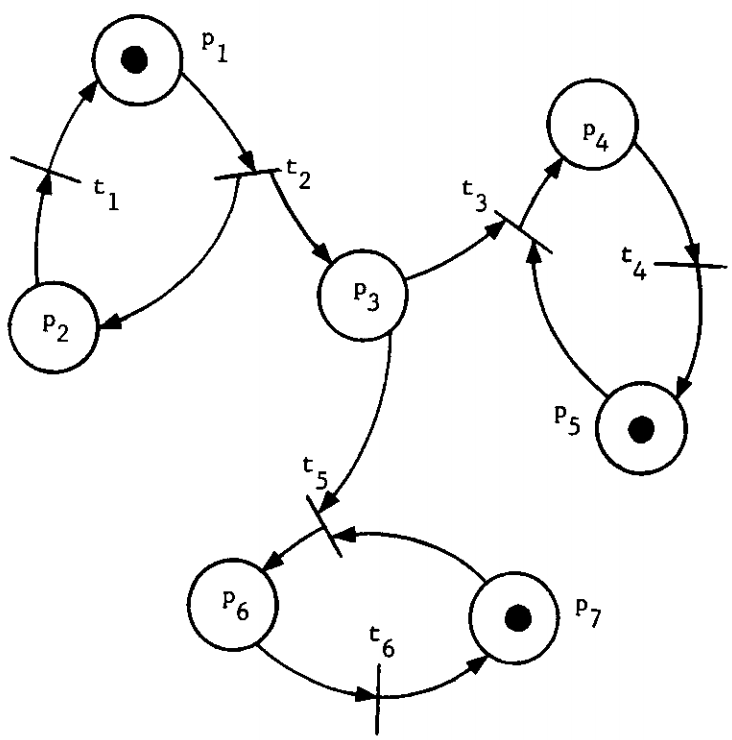
\includegraphics[width=0.8\textwidth]{pn}
\caption{Sample Petri Net, reprinted from \cite{peterson1977petri}}
\label{fig:pn}
 \end{figure}

This Petri net contains two types of nodes: circles (called \emph{places}) and
bars (called \emph{transitions}). These graph nodes are connected using directed
arcs from places to transitions and from transitions to places. If an arc is
directed from node x to node y (either from a place to a transition or a
transition to a place), then x is an input to y, and y is an input of x. In
Figure \ref{fig:pn}, place $P_2$ is an input to transition $t_1$.

In addition to static properties, a Petri net has dynamic properties that result
from its execution. The execution of a Petri net is controlled by the position
and movement of markers (called tokens) in the Petri net. Tokens, indicated by
black dots, reside in the circles representing the places of the net. A Petri
net with tokens is a marked Petri net.

Tokens are moved by the \emph{firing} of transitions of the net. A transition
must be enabled in order to fire; a transition is enabled when all of its input
places have a token in them. A transition fires by removing the enabling tokens
from their input places and generating new tokens which are deposited in the
output places of the transition. In the marked Petri net in Figure \ref{fig:pn},
the transition $t_2$ is enabled since it has a token in its input place $P_1$.
If $t_2$ fires, the token in $P_1$ is removed and a token is placed in places
$P_2$, and $P_3$.The distribution of tokens in a marked Petri net defines the
state of the net and is called a \emph{marking}. This marking may change as a
result of firing transitions. When multiple transitions are enabled for firing,
one transition is chosen randomly; the variability in the firing order of
enabled transitions enables Petri nets to model non-deterministic systems e.g.
distributed systems where the ordering of events is not well-defined or
deterministic.

Formally, a Petri net is a five tuple (P, T, A, W, $M_0$), where P is a finite
set of places, T is a finite set of transitions, A is a finite set of arcs
between places and transitions, W is a function assigning weights to arcs and
$M_0$ is some initial marking of the net. Places hold a discrete number of
markings called tokens. These tokens often represent resources in the modeled
system.

Petri nets enable the modeling and visualization of dynamic system behaviors
that include concurrency, synchronization and resource sharing. Theoretical
results and applications concerning Petri nets are plentiful
\cite{david1994petri, holloway1997survey}, especially in the modeling and
analysis of discrete event-driven systems. Models of such systems an be either
\emph{untimed} or \emph{timed} models. Untimed models are those approximations
where the order of the observed events are relevant to the design but the exact
time instances when a state transitions is not considered. Timed models,
however, study systems where its proper functioning relies on the time intervals
between observed events. Petri nets and extensions have been effectively used
for modeling both untimed \cite{holloway1997survey} and timed systems
\cite{zuberek1991timed}. For a detailed study of Petri nets and its
applications, the reader is referred to standard textbooks
\cite{peterson1977petri, reisig2012petri} and survey papers
\cite{murata1989petri, zhou1999modeling, zurawski1994petri}.

Petri nets have evolved through several generations from low-level Petri nets
for control systems \cite{reisig2012petri} to high-level Petri nets for modeling
dynamic systems \cite{jensen2012high} to hierarchical and object-oriented Petri
net structures \cite{de2001object} that support class hierarchies and subnet
reuse. Several extensions to Petri nets exist, depending on the system model and
the relevant properties being studied e.g. Timed Petri nets
\cite{wang2012timed}, Stochastic Petri nets \cite{bause1996stochastic,
marsan1994modelling} etc. High-level Petri nets are a powerful modeling
formalism for concurrent systems and have been widely accepted and integrated
into many modeling tool suites for system design, analysis and verification.

\subsection{Example High-level Petri net Tool: CPN Tools}

CPN Tools \cite{CPNTools} is an open source tool for editing, simulating and
analysis of Colored Petri nets (CPN) \cite{CPN}. A Colored Petri Net is a tuple
$(\Sigma, P, T, A, N, C, G, E, IN)$ where: $\Sigma$ ~is a finite set of
non-empty types called \textbf{color sets}. Color sets determine the types of
tokens, operations, and functions that can be used in the net inscriptions (arc
expressions, guards, etc.). \textbf{Places}, \textbf{transitions} and
\textbf{arcs} are defined by three finite sets P, T, and A respectively. N is a
\textbf{node function} $N \subseteq (P X A) U (A X P)$. The \textbf{color
function} C maps each place p into a set of possible token colors C(p) i.e. each
token on p must belong to the type C(p). The \textbf{guard function} G maps each
transition t into an expression of type boolean i.e. a predicate. The
\textbf{arc expression} function E maps each arc a into an expression which must
be of type C(p(a)) i.e. evaluation of the arc expression must yield a resultant
token that can be attached to the corresponding place. Lastly, the
\textbf{initialization function} IN maps each place p into an expression which
must be of type C(p) i.e. this function initializes each place with a token
value of the appropriate color set type. This extends the behavior of a basic
Petri net since a token represents an instance of a complex data type. In basic
Petri nets, tokens in a place can represent quantity e.g. number of tokens in a
place could indicate the number of ready threads, or tokens could represent
truthfulness of a state e.g. a token in the \emph{Blocked} place represents a
globally blocked state. In Colored Petri nets, tokens can not only represent a
much larger variety of data structures but multiple tokens in a place can have
different properties. This means that a CPN transition requires more than just
the presence of a token in its input places; the tokens must have the right data
(values) for the transition's guard conditions to be true, adding a layer of
compactness to the representation of data.

\if 0
 \fbox{\parbox{0.9\textwidth}{A \emph{Colored Petri Net} is a tuple
$(\Sigma, P, T, A, N, C, G, E, I)$ where,
 \begin{itemize}
 \item $\Sigma$ is a
finite set of non-empty types called \textbf{color sets}
 \item P is a set of
\textbf{places}
 \item T is a set of \textbf{transitions}
 \item A is a finite
set of \textbf{arcs} such that:
 \begin{itemize}
 \item $P \cap T = P \cup A = T
\cap A = \oslash$
 \end{itemize}
 \item N is a \textbf{node function}, defined
from A into $P x T \cup T x P$
 \item C is a \textbf{color function}, defined
from P into $\Sigma$
 \item G is a \textbf{guard function}, defined from T into
expressions such that:
 \begin{itemize}
 \item $\forall t \in T: [ Type(G(t)) =
Bool \wedge Type(Var(G(t))) \in \Sigma ]$
 \end{itemize}
 \item E is an
\textbf{arc expression function} defined from A into expressions such that:
\begin{itemize}
 \item $\forall a \in A: [ Type(E(a)) = C(p(a))_{MS} \wedge
Type(Var(E(a))) \in \Sigma ]$ \\
 where p(a) is a place in N(a)
 \end{itemize}
\item I is an \textbf{initialization function} defined from P into expressions
such that:
 \begin{itemize}
 \item $\forall p \in P: [ Type(I(p)) = C(p)_{MS}
\wedge Var(I(p)) = \oslash ]$
 \end{itemize}
 \end{itemize}}}
 \FloatBarrier

\vspace{0.2in}
 \fi

%CPN Tools currently supports two types of analysis for CPNs: simulation and
state space analysis. Like many simulation software packages, CPN Tools supports
single-step simulation where the Petri net is executed one transition step at a
time: on an enabled transition it causes that particular transition to occur,
while on a page it will cause a randomly selected, enabled transition on that
particular page to occur. If multiple transitions are enabled, one transition is
chosen at random, similar to Petri nets. CPN Tools also supports executing a
user-defined number of steps, where the simulation graphics will be updated
after each step. A fast-forward tool will also execute a user-defined number of
simulation steps, but without any graphics updates till after the last step.

%CPN Tools also contains facilities for generating and analyzing full and
partial (bounded) state spaces for CPN. State space analysis is discussed in
more detail in Chapter \ref{chapter:analysis} but as a summary,

%To facilitate the implementation of the state space facilities, CPN Tools uses
syntactical constraints which are important for state space generation but not
for simulation e.g. a state space cannot be generated unless all places and
transitions have unique names, and all arcs have inscriptions i.e. expressions
that evaluate to some token value. Standard state space reports can be generated
automatically and saved. Such reports contain statistical information about the
net e.g. boundedness properties, liveness properties and fairness properties.
Querying facilities enable searching a generated state space for the presence or
absence of interesting system properties.

\section{Analyzing AADL models with Petri nets}

Teams of researchers have, in the past, identified the need for in-depth timing
analysis tools that integrate with complex system design challenges, especially
in model-driven architectures \cite{kordon_sn}. Modeling languages like MARTE
\cite{MARTE:05}, which is based on UML and AADL \cite{AADL_Intro:06} provide a
high-level formalism to describe a DRE system, at both the functional and
non-functional level. MARTE (Modeling and Analysis of Real-time Embedded
Systems) defines the foundations for model-based description of real-time and
embedded systems. MARTE supports the annotation of models with information
required to perform specific types of analysis such as performance and
schedulability analysis.

In general MARTE provides a generic canvas to describe and analyze systems. The
user is required to add domain-specific and system-specific properties and
artifacts on top of the generic platform. Compared to MARTE, AADL (Architecture
Analysis and Design Language) comes with a stand-alone and complete semantics
that is enforced by the standard. In \cite{kordon_sn}, the authors propose a
bridge that translates AADL specifications of real-time systems to Petri nets
for timing analysis. This formal notation is deemed to be well-suited to
describe and analyze concurrent systems and provides a strong foundation for
formal analysis \cite{girault2013petri} methods such as structural analysis and
model checking. The high-level goal is to check and verify AADL models for
properties like deadlock-freedom and boundedness. The workflow presented here is
similar to the proposed work in this thesis in the sense that a system design
model along with user-specified properties are translated into a high-level
Petri net-based analysis model.

The execution behavior of the software in AADL is represented by AADL components
called \emph{Threads}. Interactions are modeled by communication places in the
Petri net to trigger associated actions when AADL threads receive new data (new
Petri net tokens). The thread execution is represented by an automata that has
three parts: (1) thread life cycle that handles scheduling, dispatching,
initialization and completion; (2) thread execution that executes
thread-specific code; and (3) error management that handles potential errors.
Symmetric nets \cite{hayman2008symmetry, winskel2009events} are high-level Petri
nets commonly used for analysis of causal properties in distributed systems,
where tokens can carry data and nets can have a set of initial markings.
Symmetry in a Petri net is described as a relation between its runs as causal
nets; the relation specifying when one run is similar to another. Using this
Petri net, the analysis uses model checking to verify (1) lack of deadlocks in
the system and (2) correct causality e.g. a message sent by a producer is always
received and processed by a consumer.

However, there are some potential improvements to this work. Not only is the
generated Petri net structure hard to follow, it is seemingly composed of
sub-Petri nets, one for each thread (and its lifecycle) in each process. It is
clear that although the transformation is sound, the generated Petri net models
are going to be intractably large for complicated scenarios. The state space of
the Petri net is dependent on the number of places in the net and the
corresponding internal states. The generated net would not scale well for large
process sets or distributed scenarios without using state space reduction
techniques that rely on symmetry \cite{sistla2004symmetry}. Such troubles can be
alleviated by using a high-level Petri net such as Colored Petri nets where much
more information can be packed in a Petri net token. Complex token data
structures reduce the number of places required to describe a system model e.g.
a list of C-style struct data structures can abstractly model a set of
processors. This reduces the number of places that would be required to
represent a full system. Such modeling constructs are essential in
component-based systems where the full system is typically a large assembly of
tested black box components. Lastly, the modeling constructs used are strictly
bound to AADL and cannot be easily modified for systems not modeled using AADL,
especially strictly-defined component models with precise execution semantics.

\section{Analyzing AADL Models with Timed Petri nets}

The authors in \cite{kordon_sn}, have also investigated AADL model analysis
using Petri net extensions such as Timed Petri nets \cite{kordon2009}. Using the
modeling concepts and analysis capabilities of Petri net extensions means that
developers can analyze for a larger set of system-level properties such as
schedulability dimensioning, and deadlock detection. This work allows for
efficient model-driven development and prototyping of real-time systems.

Petri nets have proven to be useful mathematical means to analyze both the
structure and behavior of a real-time system. Structural analysis involves
analyzing a model structure to obtain knowledge about properties like circular
dependencies, and causality flaws. Behavioral analysis is performed by
generating and searching a bounded state space of the system, typically deducing
safety properties e.g. deadline violations. By using Timed Petri nets, the
authors insert time into any property that needs to be verified. By tagging
these properties, state space queries reveal the temporal nature of system-level
events that enable timing analysis results e.g. worst-case response times.

The approach presented in this \cite{kordon2009} work uses a \emph{Timed Petri
net pattern} to model the thread life-cycle, derived from the corresponding AADL
model. The state of the AADL threads are modeled using places and the life cycle
is handled by the transitions. The periodicity of the thread execution is
managed external to the thread pattern, by using timed tokens that represent the
system clock. Multi-threaded execution is managed by the \emph{Processor} place.
The presence of a token in this place indicates an idle processor, enabling
potential thread state changes.

Analysis techniques using Petri nets need to record/detects errors such as
deadline violations in Petri net places. To detect missed deadlines, a
deadline-detection subnet is simply added to the TPN pattern. Similar to missed
deadlines, missed activations can also be detected. When the thread must be
dispatched but misses its activation deadline, a detector transition fires,
marking a missed activation. When model checking this system, if there is no
token in some \emph{Missed Activation} place any where in the state space of the
system, then no thread activations were missed.

Similar to this work, our Colored Petri net-based analysis work uses bounded
observer places \cite{Alpern1989} that observe the system behavior for property
violations and prompt completion of operations. However, this work
\cite{kordon2009} only considers periodic threads in systems that are not
preemptive. The non-preempt-able thread execution is evident in the need to
check for missed activations. Our analysis aims to improve on this work by (1)
generating a more scalable and efficient pattern-based analysis model and (2)
supporting various types of hierarchical scheduling algorithms, both preemptable
and non-preemptable with (3) complex periodic and aperiodic interaction
patterns.

\section{MAST: Modeling and Analysis Suite}

MAST \cite{934015} is a modeling and analysis suite for real-time applications.
MAST, still in development, aims to provide a set of tools that enable engineers
and system integrators to developing real-time applications to check the timing
behavior of their system, including schedulability analysis. The techniques
implemented by this tool focus on fixed-priority scheduled systems, such as the
ones in commercial operating systems. The tools aims to address the timing
analysis results developed for both single processor \cite{liu1973scheduling,
klein2012practitioner} and distributed real-time systems
\cite{palencia1999exploiting, tindell1994holistic}.

A model describing real-time applications should not only represent the
structure of the system but also the hard real-time requirements imposed on it.
Most of the existing schedulability analysis methods are based on a
\emph{linear} timing and interaction model where each task is activated by the
arrival of a single event or message and each message is sent by a single task.
This linear model does not allow for complex interactions e.g. nested
request-response interactions and event sequences, and so in such cases the
analysis methods are not applicable. The MAST model of real-time system is a
rich representation. It is an event-driven model where complex dependence
patterns among tasks are established e.g. tasks may be activated by the arrival
of several events at their output, making it suitable for analysis of real-time
systems designed with object-oriented methodologies. This MAST model description
is derived from a standard UML and MARTE description \cite{medina2011}.

For analysis, the MAST suite includes schedulability analysis tools that use
newly published research techniques such as the offset-based methods
\cite{palencia1998schedulability} that enhance analysis results, providing less
pessimistic estimates than previous results \cite{tindell1994holistic}. The
system description is specified through an textual description language that
serves as the input to the analysis tools. Using UML, the real-time \emph{view}
of the DRE is described \cite{selic2000generic} by adding appropriate behavior
specifying classes. The application design is linked with the real-time view to
get a full description of the modeled system, along with its timing behavior and
requirements.

\section{Verification in AutoFocus 3}

FOCUS is a general theory providing a model of computation based on the notion
of streams and stream processing functions \cite{broy2012specification}. It is
suitable to describe models of distributed, reactive systems. Based on this
mathematical foundation, a tool called AutoFocus 3 \cite{huber1996autofocus}
allows for a graphical description of systems according to this model of
computation.

In AutoFocus 3, the system model is described as a set of communicating
components. Each component has a defined interface (black box view) and an
implementation. The interface consists of a set of communication ports. A port
is either an input port or an output port, each identified by its name and its
type. Components can exchange data by sending messages through output ports and
receiving messages via input ports. Communication paths are called channels. A
channel connects an output port to some input port, thus establishing a
relationship. From the logical point of view, channels transmit messages
instantaneously.

AutoFocus 3 networks are executed synchronously based on a discrete notion of
time and a global clock. In this setting, a component can be either strongly
causal or weakly causal. A strongly causal component has a reaction delay of at
least one logical time tick which means that the current output cannot be
influenced by the current input values. A weakly causal component may produce an
output which depends on the current input i.e. the reaction is instantaneous. A
network of strongly causal components are always well defined e.g. unique
fixed-points for recursive equations induced by channel connections always
exist. Networks of weakly causal components are also well defined under the
constraint that no cycles exist i.e. no weak causal component may send a signal
that feeds back to itself in the same time tick.

Input/Output automaton models are used to define stateful component behavior.
The automaton consists of a set of control states, a set of data variables and a
state transition function. One of the control states is defined to be the
initial state of the component, while each data state variable has a defined
initial value. The state transition function is defined as a mapping from the
current state, the current input values, and the state variable values to output
values. Using this model, AutoFocus 3 supports techniques to verify the logical
architecture early in the development process e.g. automatic test case
generation and model checking. Methodologies such as in \cite{feilkas2009top}
present the application of model checking techniques to verify the logical
architecture of AutoFocus 3 models.

The formal verification process with AutoFocus 3 comprises of: (1) selecting
system parts to be verified, (2) selecting requirements for the selected parts
to be verified, (3) formally specifying the selected requirements, and (4)
formally verifying using model checking. If the model checking succeeds, then
the verification is finished, but if the model checking fails, then analysis is
required to identify the reason e.g. implementation error, requirement
formalization error etc. This analysis uses Linear Temporal Logic
\cite{gabbay1994temporal} to convert informal textual specification e.g. "The
Adaptive Cruise Control (ACC) starts by driver interaction only" to a formal
temporal logic specification using boolean and temporal operators. The system
model is exported into the modeling notation of the model checking tool SMV
\cite{mcmillan1993symbolic, mcmillan1999getting} used by the AutoFocus 3
project.

The workflow on the above verification methodology is fairly tenuous. For any
system part, a state-transition model of the part has to be constructed; this
model represents the logic working of the part. Then, all of the informal
textual requirements of the system part need to be translated into LTL
specifications by the user and then fed into the integrated model checker. One
of the reasons the model checking could fail is improper formalization of the
requirements. Secondly, the approach does not seem to model the actual execution
of the software i.e. code execution on top of layers of management software
running on appropriate hardware. Thus, the method is best utilized for
identifying logical errors in the system design or inconsistent property
specification. The approach does not necessarily model or analyze the complete
timing behavior of the component processes and is applicable mainly to early
designs where the component assembly is being prepared for integration.
 
